% !Mode:: "TeX:UTF-8"
%!TEX program  = xelatex

\documentclass{cumcmthesis}
%\documentclass[withoutpreface,bwprint]{cumcmthesis} %去掉封面与编号页
\usepackage{float}
\usepackage{url}
\usepackage[framemethod=TikZ]{mdframed}
\title{}
\tihao{B}
\baominghao{202017241008}
\schoolname{华中科技大学}
\membera{李欣航}
\memberb{鲁镇仪}
\memberc{蒋瀚锐}
\supervisor{贺云峰}
\yearinput{2020}
\monthinput{09}
\dayinput{12}

\begin{document}
\maketitle

\begin{abstract}
	\par
	\textbf{对于问题一:}

	\par
	\textbf{对于问题二:}

	\par
	\textbf{对于问题三第一小问:}

	\par
	\textbf{对于问题三第二小问:}

	\par
	\keywords{图论 \quad Dijkstra算法 \quad  }
\end{abstract}



%\tableofcontents
\section{问题重述}
\subsection{问题背景}

在日益快节奏的生活与时代的背景下,人们玩游戏的重心也逐渐的从娱乐性质转为竞争性质。
对于一款游戏来说,攻略的必要性是有目共睹的,人们越来越离不开攻略了。\par

对于这样一款益智游戏《穿越沙漠》来说,游戏内容是十分有趣的。
玩家在游戏中凭借着一张地图和其他的一些信息,就需要利用自己的智慧来完成一个又一个的选择最终到达游戏的胜利。

\subsection{问题的提出}
该文章主要是研究在《穿越沙漠》这款游戏内,在不同的六个关卡中,分别提出不同要求,不同情况下的时候,玩家所应该做的最优策略。
玩家在游戏开始时拥有一张地图,他的目标是首先在规定时间内到达终点,中途不能够使得水或食物已耗尽,并且需要能够使得最终所保留的资金尽可能多。\par

游戏本身每天有各种地点和属性,关于自然的属性分别有地点所代表区域,例如村庄,矿山;还有天气,天气分成“晴朗”、“高温”、“沙暴”这三种;关于玩家所操纵人物与人物所携带的资源的属性,分别有基础消耗量,行走消耗量,其他消耗量,水,食物以及在矿山中所能获得的资源等等。

\par
在问题一当中,这是一个单机游戏,并且给出了所有的天气状况,题目要求得到一般化结果,并给出在此情况下求出玩家所应该做出的在第一关与第二关的最优策略。

\par
在问题二当中,假设更为合理,也即玩家只知道当天的天气情况,也更加贴近现实生活。
题目要求先求出一般化结果,然后在此条件下得到玩家在第三关与第四关的最优策略。

\par
在问题三当中,游戏从单机变成了联机多人竞技,一共$n$名玩家。
若当天任意$k (2\leq k\leq n)$名玩家均是从A走到B,那么他们每个人消耗量快速增加,变成基础消耗量的$ 2k $倍。
若这$k$名玩家同时在矿山中挖矿,则每日挖矿消耗与单机时不变,仍为基础消耗量的$ 3 $倍,但所获得的收益大幅度减少,仅为基础收益的$\frac{1}{k} $。
若这$k$名玩家同一天在同一村庄中购买物品,则价格再次翻倍,也即变为原来的$4$倍。

\par
在问题三第一小问当中,事先已知每天的天气情况,每人须最初制定好决策,并且策略不可更改,题目要求得到一般化结果,并最终运用在第五关上。

\par
在问题三第二小问当中,玩家需要动态的进行下一时刻的决策方案。要求得到关于此种情况的一般化结果,并最终运用在第六关上。

\newpage
\section{问题分析}
\subsection{问题一的分析}
问题一


\subsection{问题二的分析}
问题二

\subsection{问题三的分析}
在问题三当中,



\newpage
\section{模型假设}
\begin{itemize}
	\item 认为每个地区作为一个图上的顶点进行简化处理。
	\item 将两两相邻的地区化作图种对应顶点的边进行简化处理。
\end{itemize}
\par\par\par


\section{符号说明}
\begin{table}[H]
	\caption{符号说明}
	\centering
	\begin{tabular}{ccc}
		\toprule[1.5pt]
		符号                  & 含义                                                           & 单位          \\
		\midrule[1pt]
		$w_{\mathrm{max}}$    & \qquad\qquad\quad 玩家的负载重量(waight)上限\qquad\qquad\qquad & $\mathrm{kg}$ \\
		$ m_{\mathrm{init}} $ & 玩家在特定关卡的初始资金                                       & 元(¥人民币)  \\
		$ c_w $               & 玩家在特定关卡某一天气下的基础水份(water)消耗量                & 箱            \\
		$ c_f $               & 玩家在特定关卡某一天气下的基础食物(foods)消耗量                & 箱            \\
		$ w $                 & 当天的天气(weather)                                            & 无            \\
		$ m $                 & 某一特定关卡的基础收益                                         & 元(¥人民币)  \\
		$ m_w $               & 每箱水的价格                                                   & 元(¥人民币)  \\
		$ m_f $               & 每箱食物的价格                                                 & 元(¥人民币)  \\
		$ w_w $               & 每箱水的重量                                                   & 元(¥人民币)  \\
		$ w_f $               & 每箱食物的重量                                                 & 元(¥人民币)  \\
		\bottomrule[1.5pt]
	\end{tabular}
\end{table}



\newpage
\section{地图的建模}
由于地图当中每个地区的大小跟他们的形状无关,于是可以是做一个顶点,两两相邻的区域是相邻的,可以视作一条边。
每天仅能最终从一个顶点移到另一个相邻的顶点上。
最终,此地图被化简成为无向图进行处理。\par

\begin{figure}[!h]
	\centering
	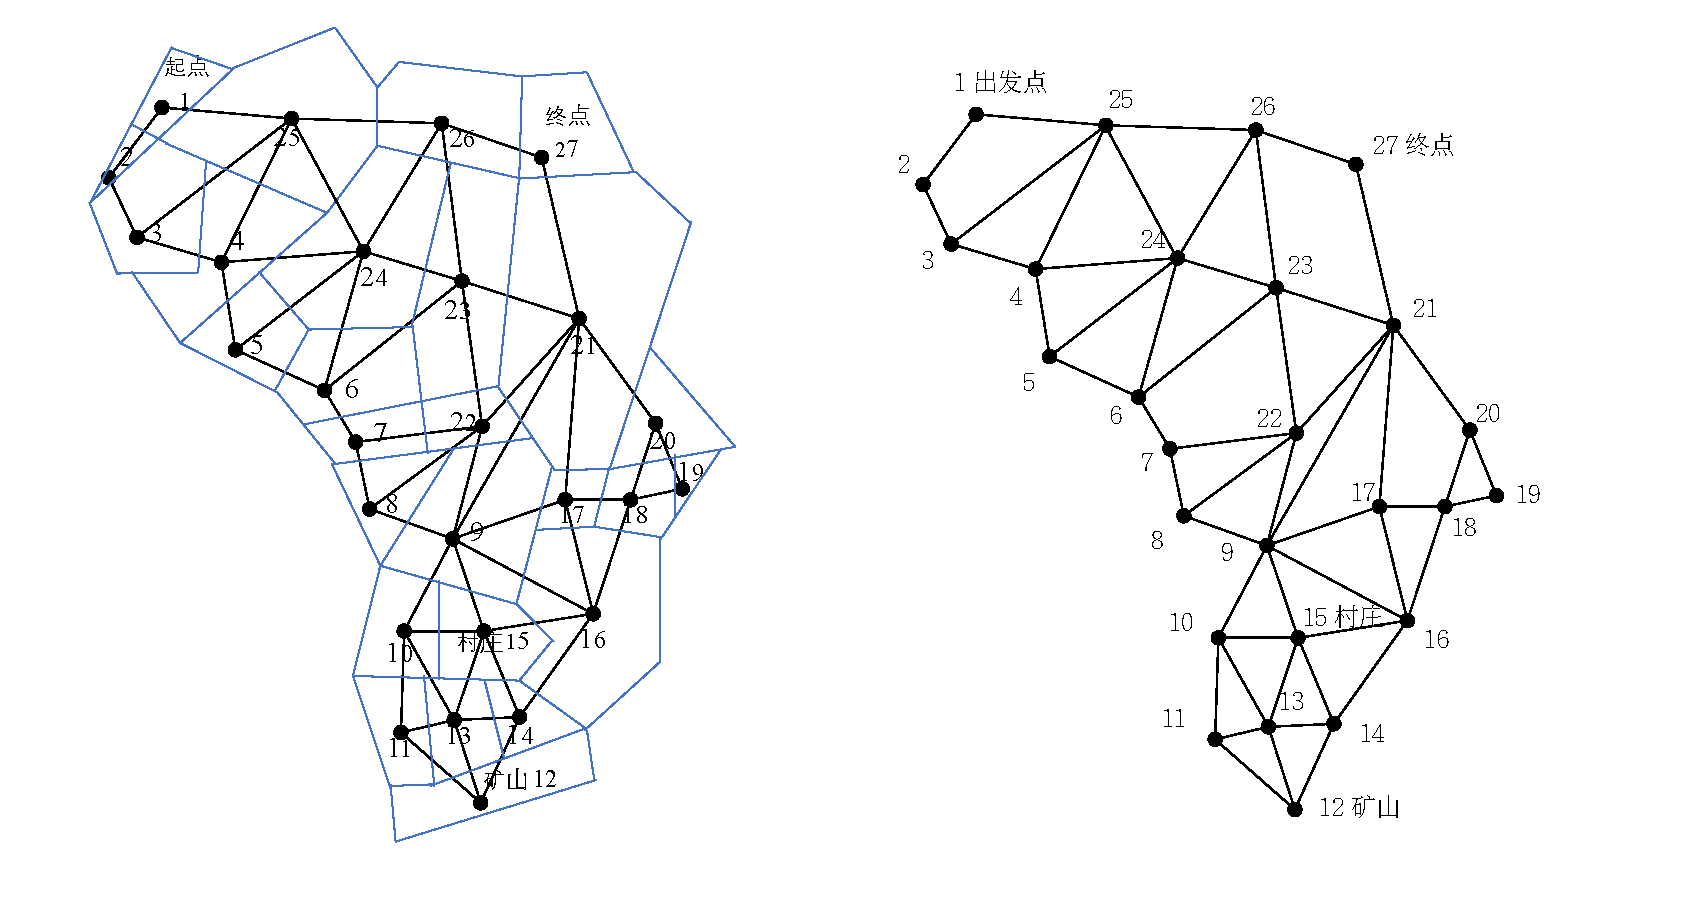
\includegraphics[width=1\textwidth]{game1-last.pdf}
	\caption{关卡一建模示意图}
\end{figure}
记这个图为$G$,此图$G$当中的所有顶点的集合记为$V$,每个地区所对应的顶点分别为$v_i\quad (1\leq i\leq |V|)$。
图$G$当中的所有边所形成的集合记为$E$,每相邻的两个地区所对应形成的边记为$e_i\quad (1\leq i\leq |E|)$,并且每个$e_i$对应着两个顶点,即$e_i=(v_j,v_k)$,其中$(v_j,v_k)$是无序点对。\par

\subsection{单机玩家选择的策略}
游戏起点的地方所对应图的点为$v_1$,游戏结束的地方所对应图的点为$v_{|V|}$。
下面不妨设$n=|V|$,也即此点为$v_n$。\par

假设村庄的分布编号为$\{a_1,a_2,\cdots,a_t\}$,矿山的编号分别为$\{b_1,b_2,\cdots,b_s\}$,利用Dijkstra算法,能够得到每一个矿山分别到起始点和终点的距离$d(v_1,v_{b_i})$和$d(v_{b_i},v_n)$。\par 

对于单位价格与重量的比较,能够发现

\begin{figure}[!h]
	\centering
	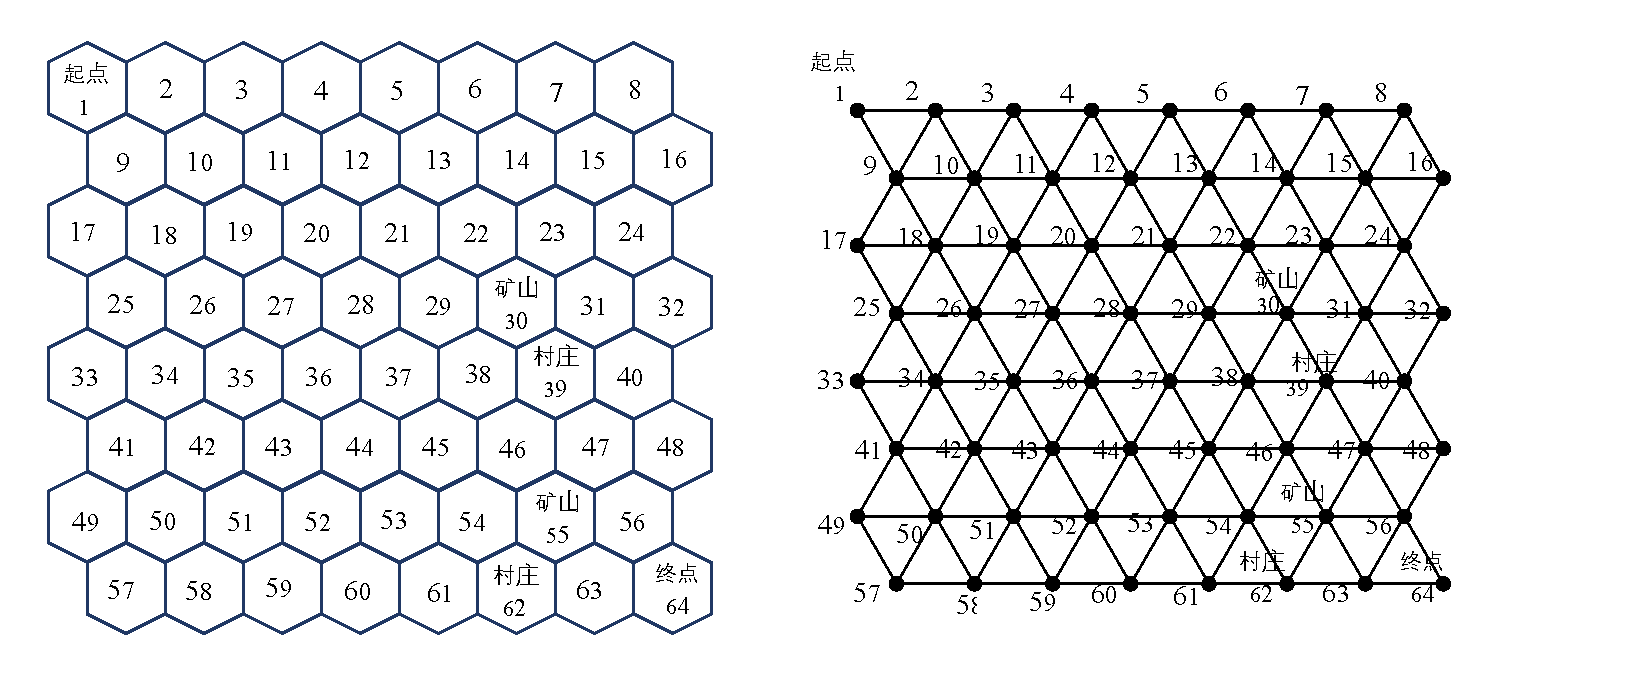
\includegraphics[width=1\textwidth]{game2-last.pdf}
	\caption{关卡二建模示意图}
\end{figure}

\begin{figure}[!h]
	\centering
	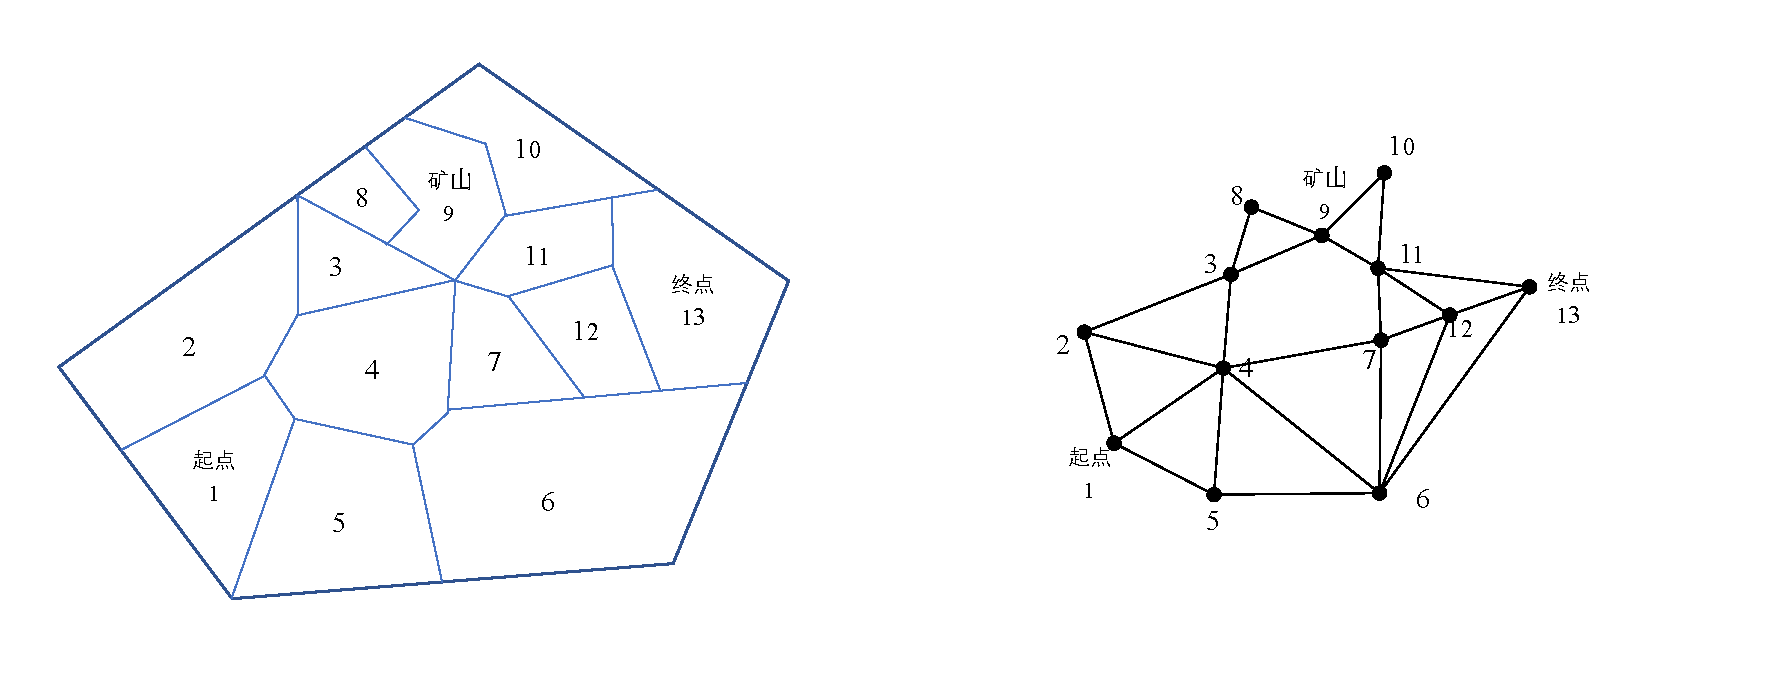
\includegraphics[width=1\textwidth]{game35-last.pdf}
	\caption{关卡三五建模示意图}
\end{figure}

\begin{figure}[!h]
	\centering
	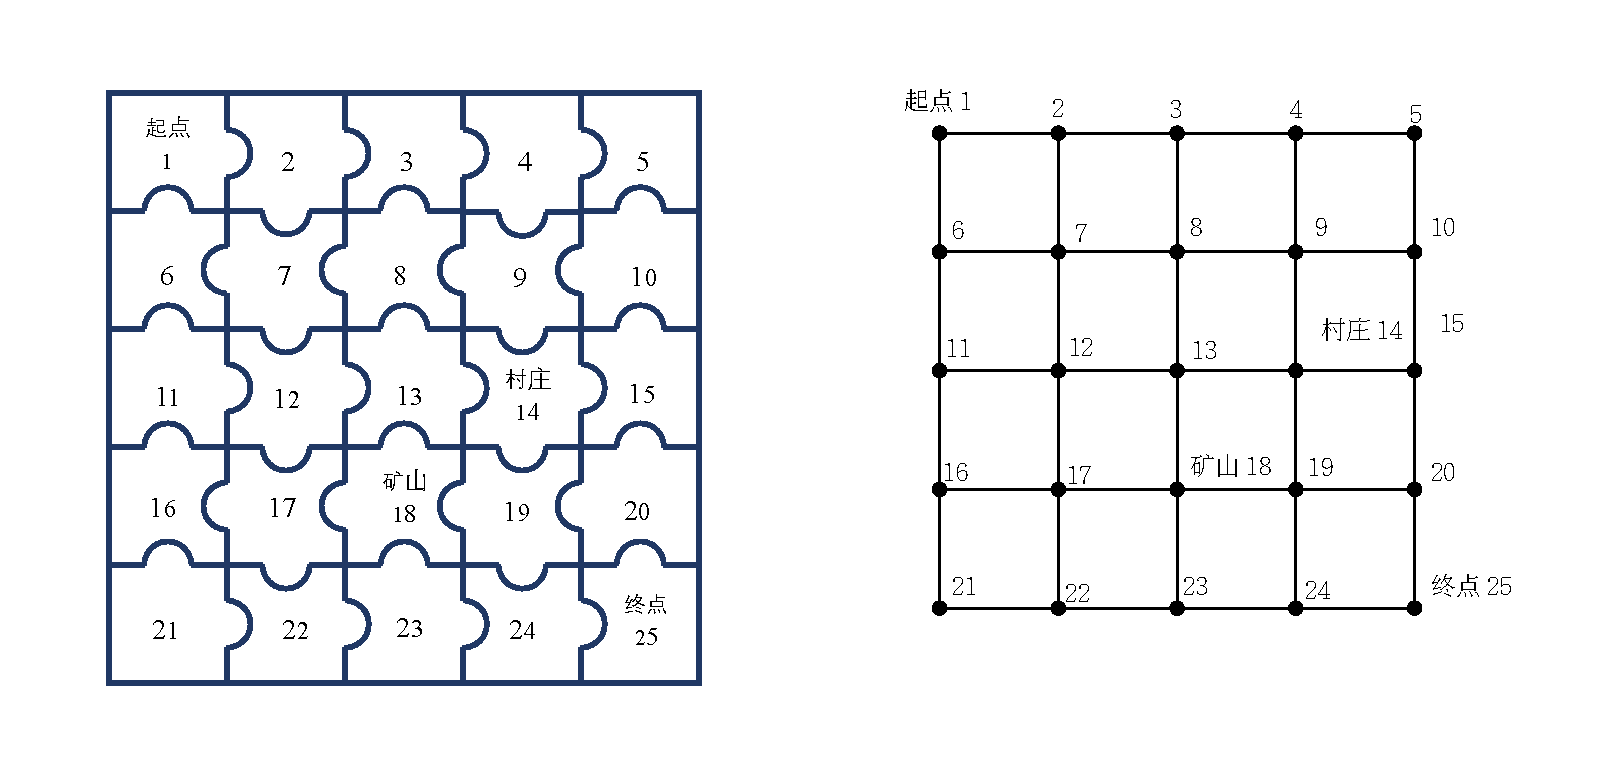
\includegraphics[width=1\textwidth]{game46-last.pdf}
	\caption{关卡四六建模示意图}
\end{figure}

\newpage
\section{模型总结}
\subsection{模型改进}

\subsection{模型的优缺点}

\textbf{模型的优点:}
\begin{itemize}
	\item[1] 问题模型
	\item[2] 问题一模型优点:
	\item[3] 问题三模型优点:
	\item[4] 问题四模型优点:
\end{itemize}

\textbf{模型的缺点:}
\begin{itemize}
	\item[1] 问题一模型缺点:
	\item[2] 问题三模型缺点:
	\item[3] 问题四模型缺点:
\end{itemize}

\newpage
%参考文献
\bibliographystyle{unsrt}%按引用的先后顺序
\bibliography{mainpaper}

\newpage
%附录
\begin{appendices}
	\section{软件版本}
	\center{MATLAB R2020a}
	\center{Python 3.8}

	\section{源程序}
	\subsection*{C++ 源代码}
	\begin{lstlisting}[language=c++]
// game12.cpp
//

#include <iostream>
#include <vector>

#define _STD ::std::

enum class weather {
	heat,
	serenity,
	sand,
};

//record the ligature situation
static const _STD vector<_STD vector<int>> map_one = {
	{},                          //0, mean nothing, ignore it.
	{2, 25},                     //1
	{1, 3},                      //2
	{2, 4, 25},                  //3
	{3, 5, 24, 25},              //4
	{4, 6, 24},                  //5
	{5, 7, 23, 24},              //6
	{6, 8, 22},                  //7
	{7, 9, 22},                  //8
	{8, 10, 15, 16, 17, 21, 22}, //9
	{9, 11, 13, 15},             //10
	{10, 12, 13},                //11
	{11, 13, 14},                //12
	{10, 11, 12, 14, 15},        //13
	{12, 13, 15, 16},            //14
	{9, 10, 13, 14, 16},         //15
	{9, 14, 15, 17, 18},         //16
	{9, 16, 18, 21},             //17
	{16, 17, 19, 20},            //18
	{18, 20},                    //19
	{18, 19, 21},                //20
	{9, 17, 20, 22, 23, 27},     //21
	{7, 8, 9, 21, 23},           //22
	{6, 21, 22, 24, 26},         //23
	{4, 5, 6, 23, 25, 26},       //24
	{1, 3, 4, 24, 26},           //25
	{23, 24, 25, 27},            //26
	{21, 26},                    //27
};

const _STD vector<int> map_one_village = { 15 };
const  _STD vector<int> map_one_mine = { 12 };

const _STD vector<enum weather> map_weather = {
	weather::heat, // nothing

	weather::heat, // the first day
	weather::heat,
	weather::serenity,
	weather::sand,
	weather::serenity,
	weather::heat,
	weather::sand,
	weather::serenity,
	weather::heat,
	weather::heat,

	weather::sand,
	weather::heat,
	weather::serenity,
	weather::heat,
	weather::heat,
	weather::heat,
	weather::sand,
	weather::sand,
	weather::heat,
	weather::heat,

	weather::serenity,
	weather::serenity,
	weather::heat,
	weather::serenity,
	weather::sand,
	weather::heat,
	weather::serenity,
	weather::serenity,
	weather::heat,
	weather::heat,
};

int Dijkstra(int x, int y, int size)
{
	_STD vector<int> ans(size, 1000000);
	ans[x] = 0;
	for (int i = 1; i < size; i++) {
		for (int j = 1; j < size; j++) {
			if (ans[j] == 1000000) {
				continue;
			}
			for (auto m : map_one[j]) {
				if (ans[j] + 1 < ans[m]) {
					ans[m] = ans[j] + 1;
				}
			}
		}
	}
	return ans[y];
}


int main()
{
	_STD cout << Dijkstra(1, 12, map_one.size()) << _STD endl;
	_STD cout << Dijkstra(12, 27, map_one.size()) << _STD endl;
}

\end{lstlisting}

\end{appendices}

\end{document}